%!TEX root = ../planets-notes.tex

\section{Trigonometric definitions}

You may remember memorizing the definitions of the sine, cosine, and tangent of an angle in a right triangle. The $\sin x$ is the ratio of the side of the triangle opposite the angle $x$ to the hypotenuse; the $\cos x$ is the ratio of the side adjacent the angle $x$ to the hypotenuse; and the $\tan x$ is the ratio of the side opposite the angle $x$ to the side adjacent the angle $x$. A useful mnemonic is \allcaps{soh-cah-toa}: Sine-Opposite-Hypotenuse --- Cosine-Adjacent-Hypotenuse --- Tangent-Opposite-Adjacent.

\begin{marginfigure}
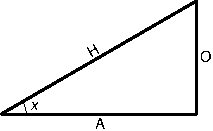
\includegraphics[width=\linewidth]{high-school-triangle}
\label{f.high-school-triangle}
\end{marginfigure}

\newthought{You may have wondered why the tangent}, for instance, is called by that name.  Now that you are a  collegiate sophisticate, we can delve more deeply into how the sine, cosine, tangent, cotangent, secant, and cosecant are constructed.
Draw a circle with a radius of unit length.  Now draw a line from the origin $O$ to intersect the circle at a point $A$, as shown in Fig.~\ref{f.trig-schematic}.  Denote by $x$ the length along the arc from the horizontal to point $A$.

From the point $A$, we draw a vertical line to the horizontal.  The length of this line $AB$ is $\sin x$. Likewise, we draw a horizontal line from point $A$ to the vertical; the length of this line, which is equal to $OB$, we call $\cos x$.  

Next, we construct a line tangent to the arc at point $A$ and extend this \newterm{tangent} to where it intersects the horizontal axis, at point $C$, and to where it intersects the vertical axis, at point $D$.  We call the length of the line $AC$ $\tan x$; the length of the line $AD$ we call $\cot x$.

\begin{marginfigure}[-6\baselineskip]
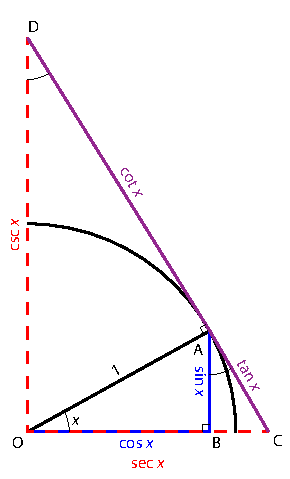
\includegraphics[width=\linewidth]{trig-schematic}
\caption[Construction from the unit circle]{Construction of the sine, tangent, secant, cosine, cotangent, and cosecant from the unit circle.}
\label{f.trig-schematic}
\end{marginfigure}

Finally, we draw from the origin $O$ lines along the horizontal to intersect the tangent at point $C$ and along the vertical to interest the cotangent at point $D$.  
The line from the origin $O$ to point $C$ is the \newterm{secant} and we call the length $OC$ $\sec x$. The line $OD$ is the \newterm{cosecant} and its length is $\csc x$.

The relationships between these quantities can be deduced by studying Fig.~\ref{f.trig-schematic}.  First, the triangle $ABC$ is similar to the triangle $OBA$. The ratio of $AC$ to $AB$ is therefore equal to the ratio of $OA$ to $OB$,
\begin{equation}\label{e.tan}
	\frac{AC}{AB} = \frac{\tan x}{\sin x} = \frac{OA}{OB} = \frac{1}{\cos x},\quad\textrm{so}
	\;\tan x = \frac{\sin x}{\cos x}.
\end{equation}
Likewise, the triangle $OAC$ is similar to $OBA$; therefore
\begin{equation}\label{e.sec}
	\frac{OC}{OA} = \frac{\sec x}{1} = \frac{OA}{OB} = \frac{1}{\cos x},\quad\textrm{so}
	\;\sec x = \frac{1}{\cos x}.
\end{equation}
Finally, the triangle $DAO$ is similar to $OBA$, giving
\begin{eqnarray}
	\frac{DO} {AO} = \frac{\csc x}{1} = \frac{OA}{BA} = \frac{1}{\sin x},&\quad&\textrm{so}
	\;\csc x = \frac{1}{\sin x},\label{e.csc}\\
	\frac{DA}{OA} = \frac{\cot x}{1} =  \frac{OB}{BA} = \frac{\cos x}{\sin x},&\quad&\textrm{so}
	\cot x = \frac{\cos x}{\sin x} = \frac{1}{\tan x}.\label{e.cot}
\end{eqnarray}
Some further relations follow immediately from the Pythagorean theorem:
\begin{eqnarray*}
	\sin^{2} x + \cos^{2} x &=& 1 \\
	\tan^{2} x + 1 &=& \sec^{2} x \\
	\cot^{x} x + 1 &=& \csc^{2} x.
\end{eqnarray*}
At small angles $x$, we see from the diagram that
$ \sin x < x < \tan x$, and $\cos x < 1$.
Further, one can show\cite{Courant1996What-is-Mathema} that
\begin{eqnarray}
	\lim_{h\to 0}\frac{\sin h}{h} = 1\quad\textrm{and}\label{e.lim-sine}\\
	\lim_{h\to 0}\frac{\cos h -1}{h} = 0.\label{e.lim-cosine}
\end{eqnarray}

\section{Trigonometric addition formulae}

To develop the formulae for $\sin(x+y)$ and $\cos(x+y)$, consider the schematic in Figure~\ref{f.trig-addition}. Here both OA and OC have unit length. The length of $OF$ is $\cos(x+y)$ and the length of $CF$ is $\sin(x+y)$.  By construction, $CE = \sin y$ and $OE = \cos y$.

\begin{marginfigure}
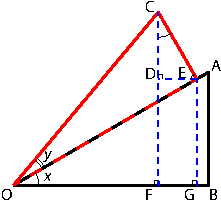
\includegraphics[width=\linewidth]{trig-addition}
\caption[Schematic of the addition of two angles]{Schematic of the addition of two angles $x$ and $y$.}
\label{f.trig-addition}
\end{marginfigure}

The length $CF = \sin(x+y)$ is the sum of $DF = EG$ and $CD$.  Now triangle $CDE$ is similar to $OBA$; hence
\[ 
	\frac{CD}{CE} = \frac{CD}{\sin y} = \frac{OB}{OA} = \frac{\cos x}{1},\quad\textrm{so}
	\;CD = \sin y\cos x. 
\]
By a similar argument, $EG = \cos y \sin x$.  Hence
\begin{equation}\label{e.sine-addition}
	CF = \sin(x + y) = \sin x\cos y + \cos x\sin y.
\end{equation}
To construct $\cos(x+y) = OF = OG-FG$, we use a similar approach to find that $FG = DE = \sin y \sin x$ and $OG = \cos y \cos x$; therefore
\begin{equation}\label{e.cosine-addition}
	\cos(x+y) = \cos x \cos y - \sin x\sin y.
\end{equation}

\section{Trigonometric derivatives}

We can now use equations (\ref{e.lim-sine}), (\ref{e.lim-cosine}), (\ref{e.sine-addition}), and (\ref{e.cosine-addition}) to establish formulae for the derivatives of the sine and cosine.  For the sine, using $\lim_{h\to 0}\sin h/h = 1$ and $\lim_{h\to 0}(\cos h - 1)/h = 0$,
\begin{eqnarray}
	\DDx{\sin x} &=& \lim_{h\to 0}\frac{\sin(x+h)-\sin x}{h}\nonumber\\
		&=& \lim_{h\to 0}\frac{\sin x\cos h + \cos x \sin h - \sin x}{h}\nonumber\\
		&=& \lim_{h\to0}\left(\cos x\frac{\sin h}{h} + \sin x\frac{\cos h-1}{h}\right) = \cos x. \label{e.dsin}
\end{eqnarray}
Likewise,
\begin{eqnarray}
	\DDx{\cos x} &=& \lim_{h\to 0}\frac{\cos(x+h)-\cos x}{h}\nonumber\\
		&=& \lim_{h\to 0}\frac{\cos x\cos h - \sin x \sin h - \cos x}{h}\nonumber\\
		&=& -\sin x. \label{e.dcos}
\end{eqnarray}
The formulae for the derivatives of the tangent, cotangent, secant, and cosecant can be derived by using the chain rule on equations~(\ref{e.tan})--(\ref{e.cot}).

\section{The Taylor Expansion}\label{s.taylor-expansion}
Suppose we wish to approximate a function $f(x)$ in the neighborhood of some point $x_{0}$ by a power series.  That it, we wish to write for some $h \ll 1$,
\[
 f(x = x_{0}+h) = c_{0} + c_{1} h + c_{2} h^{2} + c_{3} h^{3} + c_{4} h^{4}+ \ldots
\]
We assume that $f(x)$ is differentiable, and all those derivatives exist---no discontinuities or places where the derivative blows up.  To find the constants $c_{0}, c_{1}, c_{2}, c_{3}, \ldots$, we first set $h = 0$ and obtain
\[
	f(x_{0}) = c_{0},
\]
which fixes the first constant.  Next, we take the derivative and set $h = 0$, $x = x_{0}$
\[
\left.\DDx{f(x)}\right|_{x=x_{0}} = \left[c_{1} + 2c_{2} h + 3 c_{3}h^{2} + 4 c_{4} h^{3} \ldots\right]_{h= 0} = c_{1}.
\]
For the next term, we take another derivative,
\[
\left.\frac{\dif^{2}f(x)}{\dif x^{2}}\right|_{x=x_{0}} = \left[ 2c_{2} + 3\cdot 2 c_{3} h + 4\cdot 3 c_{4} h^{2}\ldots\right]_{h=0} = 2c_{2}.
\]
Thus our expansion out to the term in $h^{2}$ is
\[
 f(x_{0}+h) = f(x_{0}) + \left.\DDx{f(x)}\right|_{x=x_{0}} h + \frac{1}{2}\left.\frac{\dif^{2}f(x)}{\dif x^{2}}\right|_{x=x_{0}} h^{2} + \mathcal{O}(h^{3}).
\]
Here the expressions $\mathcal{O}(h^{3})$ means that the remaining terms are of the same size as $h^{3}$.

Applying this expansion to $\sin x$ and $\cos x$ about the point $x_{0} = 0$, we have to order $h^{2}$,
\begin{eqnarray}
	\sin h = \sin(0) + \cos(0)h - \frac{1}{2}\sin(0) h^{2} + \ldots 
		\approx h,\label{e.Taylor-sine}\\
	\cos h = \cos(0) - \sin(0) h - \frac{1}{2} \cos(0) h^{2} + \ldots
		\approx 1-\frac{h^{2}}{2}\label{e.Taylor-cosine}
\end{eqnarray}
since $\sin(0) = 0$, $\cos(0) = 1$.

